\documentclass[a4paper,12pt]{article}
\usepackage{ucs}
\usepackage[utf8x]{inputenc}
\usepackage{amsfonts}
\usepackage[english,russian]{babel}
\usepackage[T1,T2A]{fontenc}
\frenchspacing
\usepackage{amsmath,amssymb,amsthm}
\usepackage[a4paper, margin=1in]{geometry}
\usepackage[table]{xcolor}
\usepackage{multirow}
\usepackage{diagbox}
\usepackage{graphicx}
\usepackage{listings}
\usepackage[cache=false]{minted}
\graphicspath{ {./} }

\newtheorem{name}{Printed output}
\newtheorem{problem}{Задача}
\newenvironment{solution}{\renewcommand{\proofname}{\unskip\indent\nopunct}\begin{proof}}{\end{proof}}

\begin{document}

\title{ДЗ 2}
\author{Дмитрий\,Фунштейн\,гр. БИТ212}
\maketitle

\begin{problem}
    Дан файл, в котором указан рост 150 студентов. 
    Построить гистограмму с разбиением на 12 ячеек в промежутке 
    от 160 до 190 см. Найти выборочное среднее, выборочную дисперсию, 
    построить интервальную оценку для математического ожидания и дисперсии. 
    Предположим, что рост студентов подчинен нормальному распределению 
    с найденным средним и дисперсией. Построить данную функцию плотности 
    вероятности на том же графике, что и гистограмма. Проверить гипотезу 
    о том, что рост студентов распределен в соответствии с данным законом 
    распределения, с помощью критерия согласия "хи-квадрат".
\end{problem}

\begin{solution}
Выполним задание на ЯП Python с использованием библиотек Pandas, SciPy 
и NumPy. Графики будем рисовать с помощью библиотеки matplotlib через 
pyplot и средства Pandas.


\inputminted{python}{hw2.py}

\newpage
В результате исполнения написанного кода получились следующие результаты
Оценка для выборочного среднего:
$$\bar{X} = 174.35241891891891$$
Оценка для выборочной дисперсии:
$$S^2 = 30.89405296617027$$
Интервальные оценки для математического ожидания и для дисперсии:
\begin{table}[h!]
    \centering
    \begin{tabular}{|c|c|}
        \hline
        Математическое ожидание & $(173.4495082169535, 175.25532962088434)$ \\ \hline
        Дисперсия & $(24.890141243109706, 39.37900475029282)$ \\ \hline

    \end{tabular}
\end{table}
\newline
Статистика критерия хи-квадрат:
$${\chi}^2 = 3.640111044623316$$
Критическое значение хи-квадрат:
$${\chi}^2_k = 19.67513757268249$$

На основании полученных данных мы принимаем гипотезу 
о том, что рост студентов распределен в соответствии с данным законом 
распределения.

Полученная гистограмма путем исполнения программы:
\newline
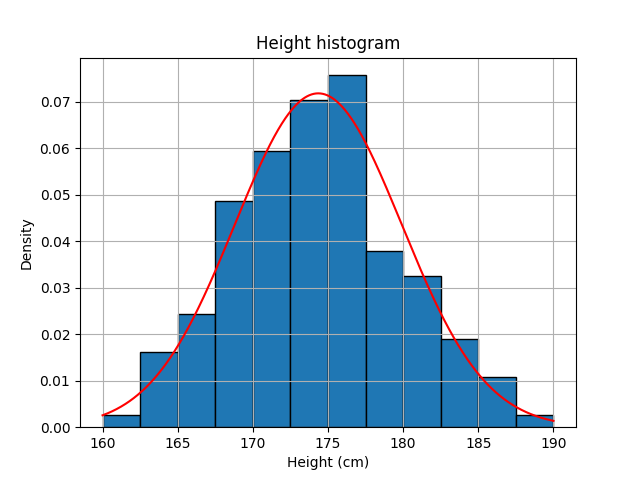
\includegraphics[width=\textwidth]{hist.png}

\end{solution}
\end{document}